\documentclass[preprint,journal]{vgtc}       % preprint (journal style)

%% Uncomment one of the lines above depending on where your paper is
%% in the conference process. ``review'' and ``widereview'' are for review
%% submission, ``preprint'' is for pre-publication, and the final version
%% doesn't use a specific qualifier. Further, ``electronic'' includes
%% hyperreferences for more convenient online viewing.

%% Please use one of the ``review'' options in combination with the
%% assigned online id (see below) ONLY if your paper uses a double blind
%% review process. Some conferences, like IEEE Vis and InfoVis, have NOT
%% in the past.

%% Please note that the use of figures other than the optional teaser is not permitted on the first page
%% of the journal version.  Figures should begin on the second page and be
%% in CMYK or Grey scale format, otherwise, colour shifting may occur
%% during the printing process.  Papers submitted with figures other than the optional teaser on the
%% first page will be refused.

%% These three lines bring in essential packages: ``mathptmx'' for Type 1
%% typefaces, ``graphicx'' for inclusion of EPS figures. and ``times''
%% for proper handling of the times font family.

\usepackage{mathptmx}
\usepackage{graphicx}
\usepackage{times}
\usepackage{color}
\usepackage{bm}
\usepackage{amsmath}

%% We encourage the use of mathptmx for consistent usage of times font
%% throughout the proceedings. However, if you encounter conflicts
%% with other math-related packages, you may want to disable it.

%% allow for this line if you want the electronic option to work properly
\vgtcinsertpkg

%% Paper title.

\title{Muscular fascicle arrangement based on Laplacian vector fields}

%% This is how authors are specified in the journal style

%% indicate IEEE Member or Student Member in form indicated below
\author{Jan Kusterer, Niven Ratnamaheson, Raimund Rolfs, and Tobias Walter}
\authorfooter{
%% insert punctuation at end of each item

}

%other entries to be set up for journal
%\shortauthortitle{Schmid \MakeLowercase{\textit{et\,al.}}: ProjINF for fun and profit}

%% Abstract section.
\abstract{
} % end of abstract

%% Keywords that describe your work. Will show as 'Index Terms' in journal
%% please capitalize first letter and insert punctuation after last keyword
\keywords{muscle, fascicle, mesh, Laplacce, electrostatic, streamline}

%% ACM Computing Classification System (CCS).
%% See <http://www.acm.org/class/1998/> for details.
%% The ``\CCScat'' command takes four arguments.

\CCScatlist{ % not used in journal version
	\CCScat{Computer Graphics}{I.3.8}{Applications}{Molecular Dynamics Visualization}
	\CCScat{Simulation and Modeling}{I.6.6}{Simulation Output Analysis}{Molecular Dynamics Visualization}
	\CCScat{Computer Graphics}{I.3.7}{Three-Dimensional Graphics and Realism}{Raytracing}
}

\graphicspath{{pics/}}

%% Uncomment below to include a teaser figure.
%\teaser{
%\centering
%\includegraphics[width=12cm]{teaser}
%\caption{blah
%}\label{fig:teaser}
%}

%%%%%%%%%%%%%%%%%%%%%%%%%%%%%%%%%%%%%%%%%%%%%%%%%%%%%%%%%%%%%%%%
%%%%%%%%%%%%%%%%%%%%%% START OF THE PAPER %%%%%%%%%%%%%%%%%%%%%%
%%%%%%%%%%%%%%%%%%%%%%%%%%%%%%%%%%%%%%%%%%%%%%%%%%%%%%%%%%%%%%%%%

\begin{document}

%% The ``\maketitle'' command must be the first command after the
%% ``\begin{document}'' command. It prepares and prints the title block.

%% the only exception to this rule is the \firstsection command
\firstsection{Introduction}\label{sec:intro}
%
\maketitle
%
%% \section{Introduction} %for journal use above \firstsection{..} instead
%
%\todo{Cite some stuff: bullshit~\cite{lipsa2011visualization} and simulation~\cite{hocker:084707}.}
%
\section{Reassembling}
The stl-file doesn't connect the surface triangles with its neighbours. Gmesh however needs one big surface to create a volume in which we can compute the streamlines. To connect all the small surfaces, we use the reclassify option with a threshold of 0. This runs an edge-detection for all triangles with an angle to its neighbour greater than 0°. This excludes the two cut surfaces, since these surfaces all have an angle of 0°. Finally we can recombine all the detected surfaces to one big surface.

With this new reassembled 3D-structure we now run our python script to detect the two cut surfaces. Since we cut the biceps orthogonal to the Z-axis the process is fairly simple. We look for all vertices with the highest z-coordinate for the upper boundary and the lowest z-coordinate for the lower boundary, respectively. These two sets are grouped and form two new surfaces. With this surface we save the maximum and minimum of the y- and x- coordinates for later use of the streamlines. We do this to cover the whole surface with the starting points of thestreamlines.(bearbeitet)

\section{Meshing}
Meshing with Gmsh is fairly easy. On default gmsh selects between three 2D algorithms and two 3D algorithms.
The automatic algorithm selection tries to select the most apropriate for the given structure.
For 2D algorithms there are "MeshAdapt", "Delauny" and the "Frontal" algorithm. Every one of them has different uses. According to Gmsh The "MeshAdapt" works best for very complex, curved surfaces. "Frontal" is the best choice, when high element quality is important. And "Delauny" is fastest for large meshes of plane Surfaces.
As stated in the manual for Gmsh the automatic selection chooses "Delauny" for plane surface and "MeshAdapt" for all other surfaces. 
For 3D algorithms there are "Delauny" and "Frontal". The “Delaunay” algorithm is the most robust and the fastest. However, this algorithm will sometimes modify the surface mesh, and is thus not suitable for producing hybrid structured/unstructured grids. In that case the “Frontal” algorithm should be preferred. As our mesh is only unstructured, the "Delauny" is our algorithm. The quality of the elements produced by both algorithms is comparable.
For our 3D Mesh, first, the 2D surfaces, then the Volume is meshed.
\begin{figure}
	\begin{center}
		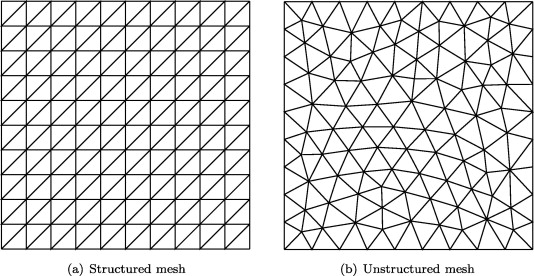
\includegraphics[width=\linewidth]{gridCompare.jpg}
	\end{center}
	\caption{Comparisson of structured and unstructured grids ~\cite{}}
	
\end{figure}
%-------------------------------------------------------------------------
\section{Simulation}
Our goal is to calculate streamlines, which according to ~\cite{choi2013} are close to 
equal to muscle fascicles. Gmsh's solver getDP features a plugin, which calculates the Streamlines based on the Laplacian vector field. Therefore we need a simulation on fluid flow or Electrostatics. The Laplace equation can be used in 3D just as in 2D. getDP's problem definition files (.pro) are used to descripe the models for simulation. In this model we consider the calculation of the electric field given a static distribution of electric potentiol. This matches to an "electrostatic" physical model. On the one End of the Muscle we have a conducting surface on top of a dielectric Volume, called "Body". A Dirichlet boundary sets the potential on the boundary of the conducting surface , called "Electrode", to 10 mV and to 0 V on the other end of the Muscle, called "Ground".
A homogeneous Neumann boundary condition is definded on the surface of the muscle to truncate the domain.\newline
The Structure of the File is as Follows:
\begin{description}
	\item[Group]
	start by giving meaningful names to physical regions defined in the mesh file.
	We only use the Regions Body, Electrode and Ground. After that we define abstract regions, that are used below.
	\item[Function]
	Here we define Material laws.
	\item[Constraint]
	The Dirichlet boundary condtition is defined piecewise. The constraint "Dirichlet\_Ele" is invoked later in the FunctionSpace.
	\item[Group]
	This is the domain definition of The FunctionSpace, which lists al regions on wich a field is defined. The Domain contains both the Volume and the Surface of the muscle.
	\item[FunctionSpace]
	The functionSpace is used to pick the electric scalar potential. The solution is defined  by:\newline
	-the domain defenition\newline
	-a type\newline
	-a set of basis functions\newline
	-a set of entities to wich the basis functions are associated (here all the nodes of the domain)\newline
	-a constraint (here the Dirichlet boundary conditions)\newline
	\item[Jacobian]
	
\end{description}
\section{Streamlines}
So now we use the earlier mentioned Plugin, which calculates Streamlines. The starting points of the Streamlines are on the upper surface of the biceps, which was calculated in the Reassembling section. The number of Streamlines can be calculated by multiplying the x- and y- coordinates from the mentioned surface. Afterwards instead of extracting the complete streamlines, we can only extract the stepwise vector data of the streamlines into a postprocessing file in our case this is called BicepsStreamline.pos.

\section{Representation of Data}
Our next step is to add up the vectors of each streamline separately. This is done by our Python Script Streamline-converter, which gets the vector data from the BicepsStreamline.pos file. Furthermore, the script creates a new file streamlines.geo with the data of each streamline in it. All in all, we can now use GMSH to merge the streamlines.geo file with our biceps surface to visualize the result.
%% if specified like this the section will be ommitted in review mode
\acknowledgments{
This work was partially funded by cake and coffee.
}

\bibliographystyle{abbrv}
%%use following if all content of bibtex file should be shown
%\nocite{*}
\bibliography{template}
\end{document} 